\documentclass[a4paper, 12pt]{article}
\usepackage[usenames,dvipsnames,svgnames,table]{xcolor}
\usepackage[T1]{fontenc}
\usepackage{times}
\usepackage[utf8]{inputenc}
\usepackage{wallpaper}
\usepackage[absolute]{textpos}
\usepackage[top=2cm, bottom=2.5cm, left=3cm, right=3cm]{geometry}
\usepackage{sectsty}
\sectionfont{\fontsize{14}{15}\selectfont}
\subsectionfont{\fontsize{12}{15}\selectfont}
\subsubsectionfont{\fontsize{12}{15}\selectfont}
\usepackage{algorithm}
\usepackage[noend]{algpseudocode}
\usepackage{listings}
\usepackage{amsmath}
\usepackage{amsfonts}
\usepackage[hang]{footmisc}

\definecolor{MyDarkGreen}{rgb}{0.0,0.4,0.0} % This is the color used for comments
\lstloadlanguages{AVR}%
\lstset{language=AVR, % AVR 8-bit Assembler
        basicstyle=\tiny,
        literate={å}{{\ra}}1
                 {ä}{{\"a}}1
                 {ö}{{\"o}}1,
        keywordstyle=\color{Blue}\bf, % Instructions in blue, bold
        keywordstyle=[2]\color{Orange}, % Registers and ports in orange
        keywordstyle=[3]\color{Purple}, % Directives in purple
        commentstyle=\color{MyDarkGreen},
        tabsize=4, % 5 spaces per tab
        numbers=left, % Line numbers on left
        firstnumber=1, % Line numbers start with line 1
        numberstyle=\tiny\color{Blue}, % Line numbers are blue and small
        stepnumber=1 % Line numbers go in steps of 5
}

% Creates a new command to include an asm script,
% the first parameter is the filename of the program (without .asm),
% the second parameter is the caption
\newcommand{\avrasm}[2]{
\begin{itemize}
\item[]\lstinputlisting[caption=#2,label=#1]{#1}
\end{itemize}
}

\newsavebox{\mybox}
\newlength{\mydepth}
\newlength{\myheight}
\newenvironment{sidebar}
{\begin{lrbox}{\mybox}\begin{minipage}{\textwidth}}
{\end{minipage}\end{lrbox}
 \settodepth{\mydepth}{\usebox{\mybox}}
 \settoheight{\myheight}{\usebox{\mybox}}
 \addtolength{\myheight}{\mydepth}
 \noindent\makebox[0pt]{\hspace{-20pt}\rule[-\mydepth]{1pt}{\myheight}}
 \usebox{\mybox}}

\newcommand\BackgroundPic{
    \put(-2,-3){
    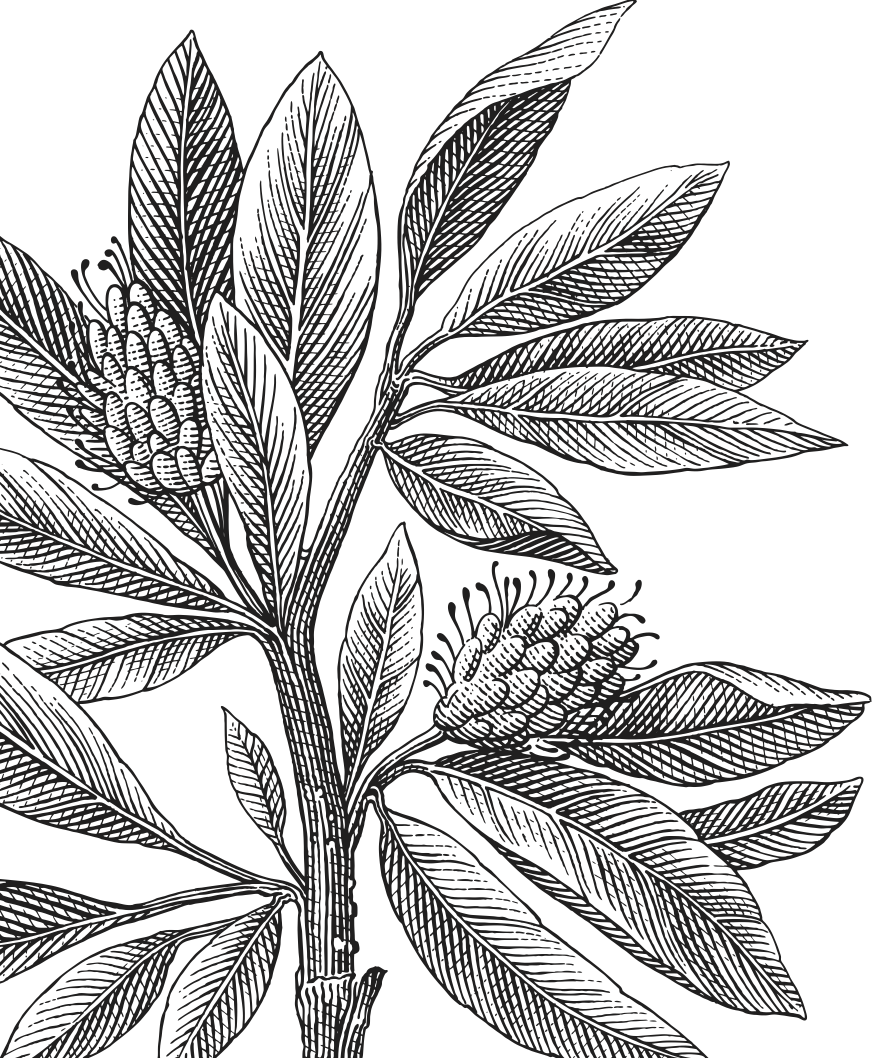
\includegraphics[keepaspectratio,scale=0.3]{lnu_etch.png} 
    }
}
\newcommand\BackgroundPicLogo{
    \put(30,740){
	
\includegraphics[keepaspectratio,scale=0.10]{logo.png}     
    }
}

\title{	
\vspace{-8cm}
\begin{sidebar}
    \vspace{5cm}
    \normalfont \normalsize
    \Huge Report \\
    \vspace{-1.3cm}
\end{sidebar}
\vspace{3cm}
\begin{flushleft}
    \huge Laboratory 4\\  
\end{flushleft}
\null
\vfill
\begin{textblock}{6}(10,13)
\begin{flushright}
\begin{minipage}{\textwidth}
\begin{flushleft} \large
	\emph{Author:} \\ Caroline Nilsson \textit{(cn222nd)} \\ Daniel Alm Grundström \textit{(dg222dw)} \\
	%\emph{Handledare:} \\ 
	\emph{Term:} HT 2017\\ 
	\emph{Course:} 1DT301 - Computer Technology I\\
\end{flushleft}
\end{minipage}
\end{flushright}
\end{textblock}
}
\date{\today} 

\begin{document}

\pagenumbering{gobble}
\newgeometry{left=5cm}
\AddToShipoutPicture*{\BackgroundPic}
\AddToShipoutPicture*{\BackgroundPicLogo}
\maketitle
\restoregeometry
\clearpage

\pagenumbering{gobble}

\tableofcontents
\newpage
\pagenumbering{arabic}



\section{Assignment 1}


\begin{figure}[h]
\centering
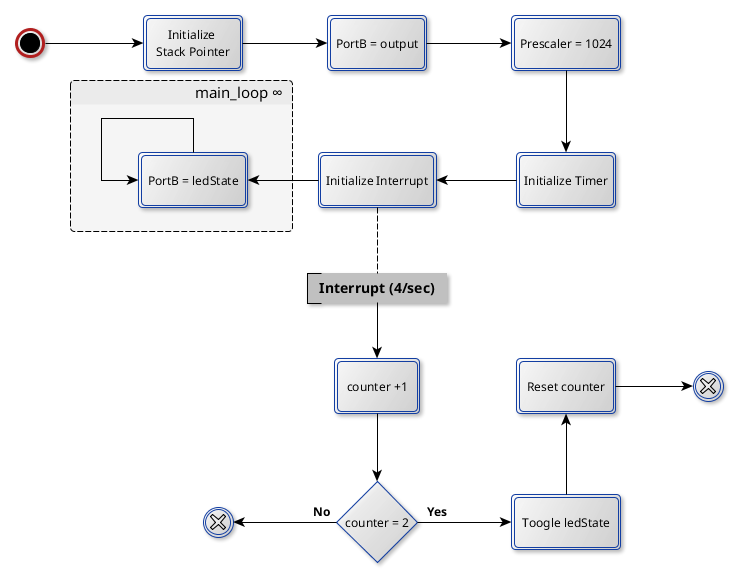
\includegraphics[scale=0.5]{flowcharts/a1_flowchart.png} 
\caption{Generate 1 Hz square wave with duty cycle 50\%}
\label{assign1.flow}
\end{figure}

\avrasm{../src/a1.asm}{}
\newpage

\section{Assignment 2}

\begin{figure}[h]
\centering
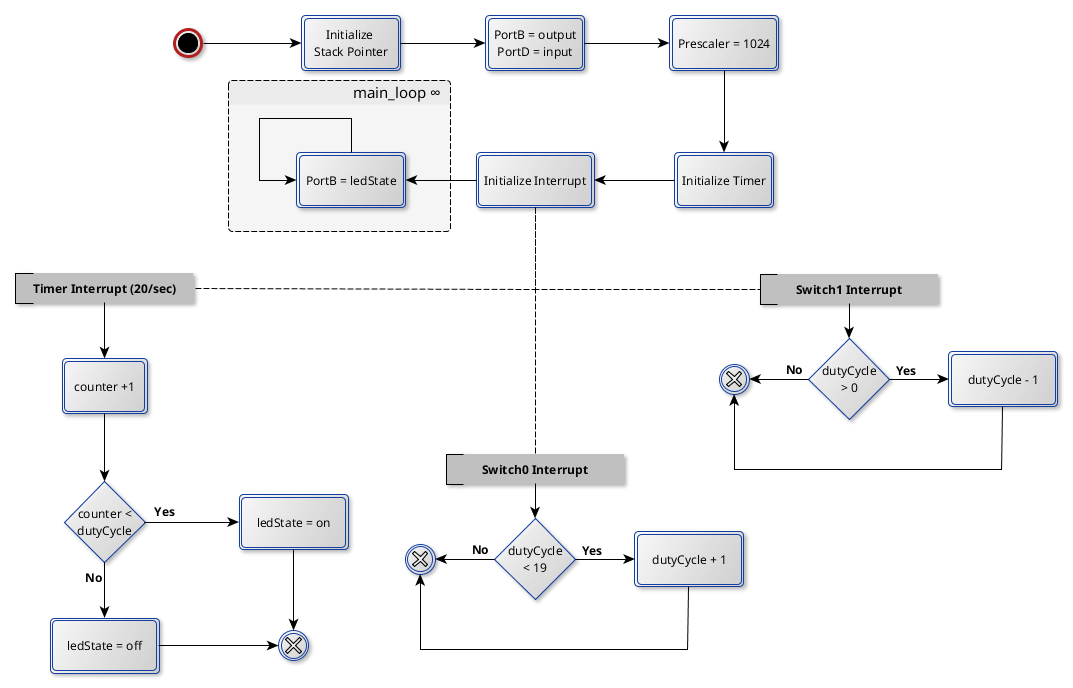
\includegraphics[scale=0.35]{flowcharts/a2_flowchart.png} 
\caption{Generate 1 Hz square wave with variable duty cycle 0\%-100\%}
\label{assign2.flow}
\end{figure}

\avrasm{../src/a2.asm}{}
\newpage

\section{Assignment 3}

\begin{figure}[h]
\centering
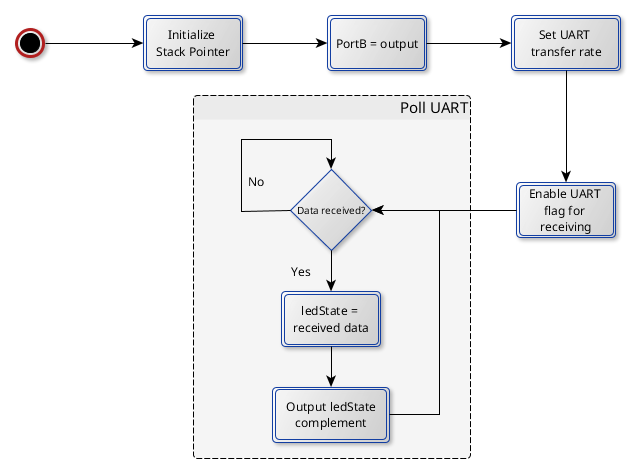
\includegraphics[scale=0.5]{flowcharts/a3_flowchart.png} 
\caption{Poll UART and output binary ascii}
\label{}
\end{figure}

\avrasm{../src/a3.asm}{}
\newpage

\section{Assignment 4}

\begin{figure}[h]
\centering
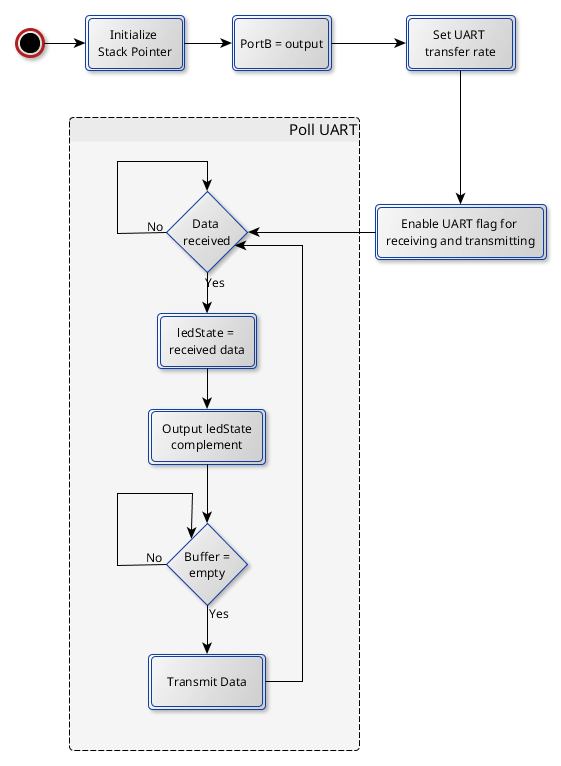
\includegraphics[scale=0.4]{flowcharts/a4_flowchart.png} 
\caption{Poll UART, output binary ascii and echo}
\label{}
\end{figure}

\avrasm{../src/a4.asm}{}
\newpage

\section{Assignment 5}
\begin{figure}[h]
\centering
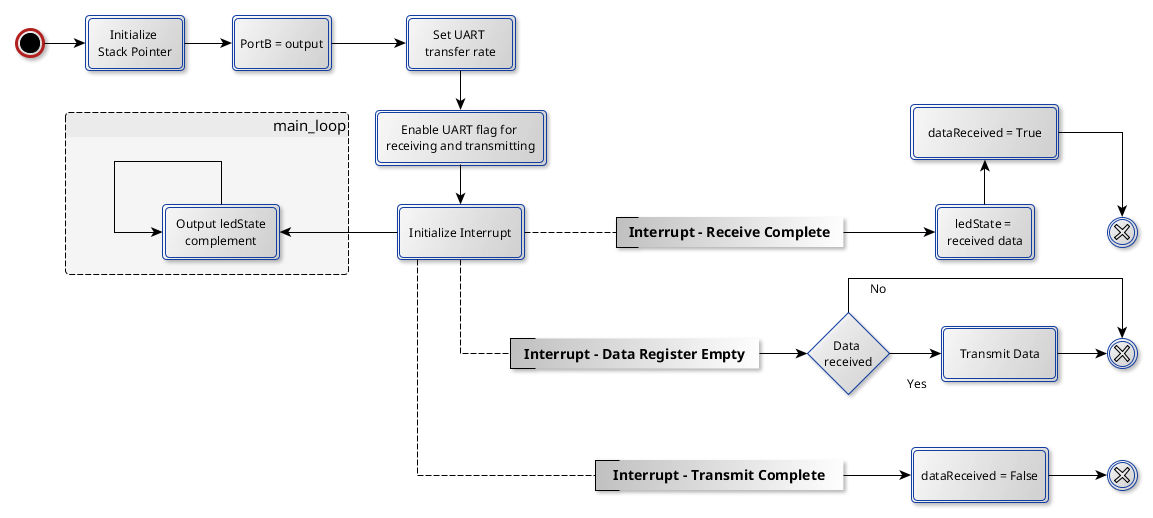
\includegraphics[scale=0.35]{flowcharts/a5_flowchart.png} 
\caption{Read UART, output binary ascii and echo. Using interrupts.}
\label{}
\end{figure}

\avrasm{../src/a5.asm}{}
\newpage

\end{document}
